Outdoorové hry často mají nějaký příběh, který se dá vyprávět konkrétními úkoly na stanovištích.
Na některých stanovištích proto musí být lidská obsluha, na jiných ale může být lidská obsluha z příběhového pohledu nežádoucí.
Když má hráč například vyřadit automatický bezpečnostní systém je lidská obsluha stanoviště poslední možnost.
Podobná stanoviště proto bývají realizovány pomocí různých papírků a provázků.
To určitě má své kouzlo, ale i tak je u podobného stanoviště vhodné mít obsluhu.
Elektronické řešení podobných stanovišť by ale mohlo otevřít úplně nový svět možností.

%% Položme si tedy otázku, jak by takové zařízení mohlo vypadat.
Podstatný fakt je, že prakticky všichni u sebe dnes mají chytrý telefon, čehož můžeme využít.
Nemá proto velký význam, aby toto zařízení suplovalo funkce telefonu.
Např. grafický výstup typu display proto v podobném zařízení není potřeba, a v tomto směru už odvádí telefon naprosto dostatečnou práci.
Pokud by tedy v rámci hry bylo potřeba například předat hráči nějaký text nebo obrázek, může jej zařízení poslat uživateli na telefon.
Možnost propojení s telefonem je také velmi významná při nastavování hry.
Díky telefonu totiž zařízení nepotřebuje uživatelské rozhraní přizpůsobené nastavování.

Mohlo by se zdát, že herní stanoviště vlastně ani není potřeba a stačila by mobilní aplikace.
Ale přestože je mobil ve hrách dobře využitelný, jsou aplikace, na které jednoduše vhodný není.
Pokud má hráč například ze stanoviště získat nějaký fyzický objekt, mobil neposlouží.
Pro hráče ani organizátory také nemusí být zrovna komfortní před hrou zařizovat, aby měli všichni nainstalovaný správný software.
% Telefon také není například na stanovišti v lese dobře viditelný.
V neposlední řadě jde také o jistý "cool efekt", který běžné zařízení jako mobil nebo třeba tablet neposkytne. %%TODO: tohle chce nějak přeformulovat

Zařízení určené primárně pro outdoorové hry bychom mohli rozdělit na dvě skupiny, statické a dynamické, protože jsou na tyto skupiny kladeny výrazně jiné požadavky.
Dynamická zařízení jsou ta, která může uživatel pohodlně nosit s sebou.
Do dynamických zařízení by se tak dal zařadit právě i telefon, ten však může být z různých důvodu nevhodný a proto i tato zařízení dává smysl navrhnout specificky pro hry.
Statické zařízení je naopak zařízení, u kterého se nepředpokládá, že jej bude hráč nosit s sebou.
Přesto by mělo být jednoduše přenositelné, má jít o stanoviště, které se jednoduše donese na své místo a během hry se s ním nebude pohybovat.
Takové zařízení by tedy mělo být dobře viditelné a splňovat požadavky, které na něj konkrétní hra klade. %%TODO: tohle chce nějak přeformulovat?
Požadavky různých her můžou být ale dost rozdílné, častým požadavkem je něco uchovávat a např. po zadání hesla hráči vydat.
Hra ale taky může vyžadovat, aby bylo zařízení sto přehrát nějakou audio nahrávku nebo naopak pořídit záznam. %%TODO: tohle chce nějak přeformulovat?
Z těchto důvodů považujeme za vhodnější zařízení koncipovat jako základní řídící jednotku, která je samostatně funkční a použitelná při hře, ale ke které se dají jednoduše připojit moduly pro konkrétní herní mechaniky.

\section{Základní řídící jednotka}
% Z toho plyne otázka, jaká funkcionalita je potřebná v základním zařízení?
Asi žádný systém, se kterým hráč přímo interaguje, není nutný v každé hře.
Jde tedy o to vybrat takové systémy, které svými nároky nepřevýší užitečnost při hrách.
Ze zkušeností považujeme za nejzákladnější systém nějaký světelný výstup, ten dokáže většinu her velmi příjemně ozvláštnit.
Většinou je nezbytný i nějaký uživatelský vstup, na což většinou stačí obyčejná tlačítka.
Problém je ale určit jaké a kolik jich bude potřeba.
Některé hry vyžadují třeba jen jedno, ale takové, aby se do něj dalo co nejpohodlněji praštit v běhu, protože je zrovna cílem ke stanovišti co nejrychleji doběhnout.
Jiná hra může vyžadovat tlačítek víc, ale už není potřeba, aby byly tak velké, protože hráč při jejich používání nebude tak akční, ale bude třeba zadávat výsledek nějakého logického úkolu.
Univerzálnější je tedy nepoužívat tlačítka, ale nějaký systém, který se dá softwarově přizpůsobit.
Příkladem může být dotyková plocha, která se dá softwarově rozdělit na různé oblasti sloužící jako tlačítka a i během hry se tak dá počet tlačítek měnit.
Další důležitou vlastností je možnost komunikace s ostatními zařízeními, která do hry přináší novou možnost jak stanoviště propojit a také pohodlnou metodu jak stanoviště nastavit přes telefon.
V neposlední řade je potřeba nějaký zvukový výstup, který může být použit např. jako potvrzení zadaného hesla.

Z toho nám tedy plyne diagram \ref{fig:diagram_zanoreni_0}.
\begin{figure}[h]
    \centering
    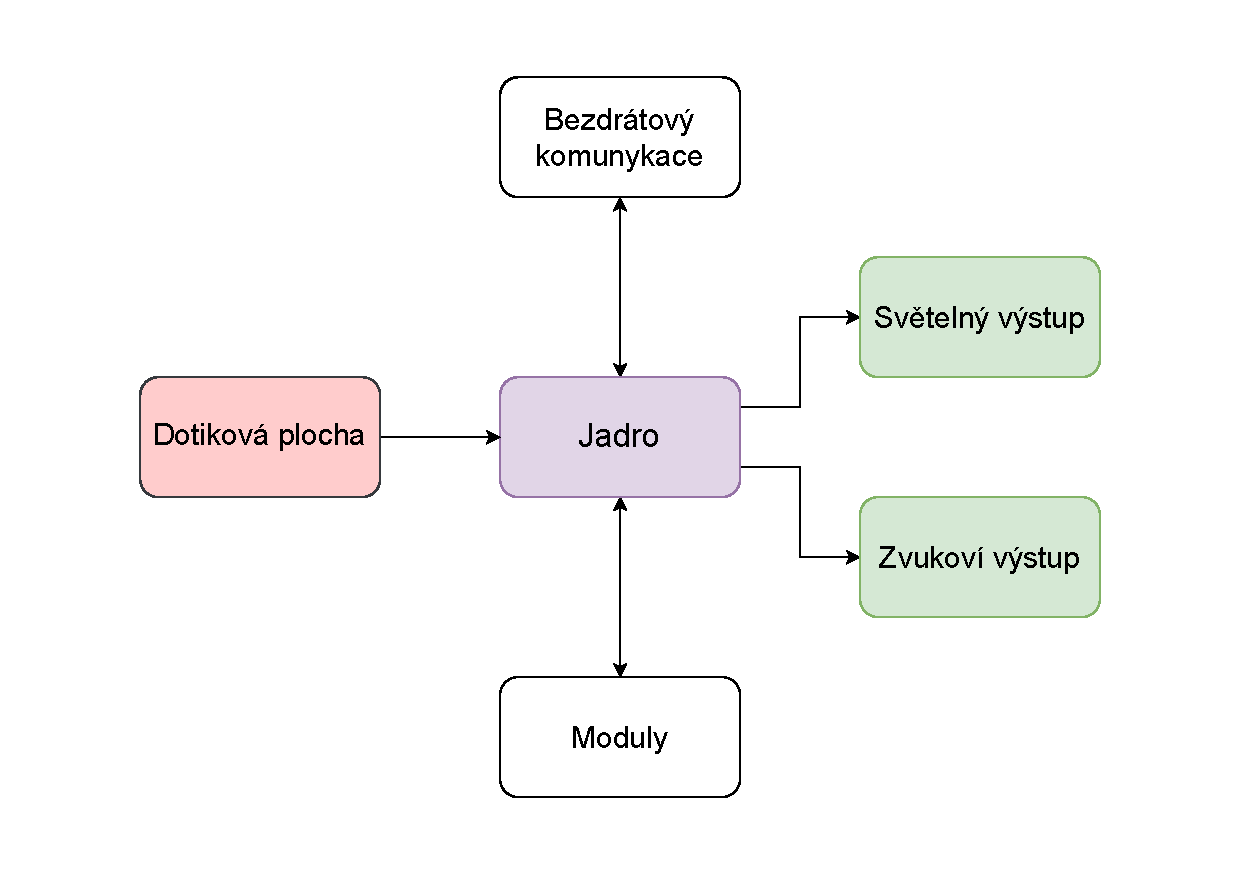
\includegraphics[width=0.65\textwidth]{text/TeoretickyUvod/AplikaceHernichZarizeni/diagram/zanoreni_0.pdf}
    \caption{Úvodní blokové schéma zařízení}
    \label{fig:diagram_zanoreni_0}
\end{figure}

\newpage

Co se světelného výstupu týče, na signalizaci různých stavů je vhodné používat různé barvy světel.
% Jaký vzhled by ale měl mít zdroj barevného světla na podobném zařízení?
Jak je uvedeno výše, není potřebné suplovat grafický display, za tímto účelem se dá použít propojení s telefonem.
Informace, kterou by zařízením mohlo často poskytovat je čas a směr, např. čas do konce kola nebo směr k dalšímu úkolu.
Podobné informace se dají elegantně zobrazit na kruhu.
Protože má být stanoviště viditelné i z větší vzdálenosti, je tedy otázkou, zda použít jen jeden kruh, tak aby byl dostatečně viditelný, nebo jich použít více. %%TODO: otázka co s totu otázkou?
Zobrazování pracuje ve dvou režimech, čtení na dálku a čtení na blízko.
Pro čtení na blízko je cílem přímá interakce se zařízením např. už zmiňované zadávání hesla.
Čtení na dálku je naopak určeno pro předávání informací hráči, když právě přímo neinteraguje se stanovištěm, např. který tým má zrovna povolený přístup.
Proto je vhodné mít kruhů víz, aby bylo možné zobrazovat tyto informace na různých kruzích, které mohou navíc být svému účelu přizpůsobeny.
Jeden kruh tak může svítit jen jedním směrem aby ho hráč vyděl celí najednou pro blízkou interakci, zatímco druhý kruh může svítit do všech stran aby byl vidět z co nejvíce míst.

Potřeba propojení s telefonem nám omezuje možnosti co se týče bezdrátové komunikace, protože telefony jsou většinou vybavený Bluetooth a WiFi.
Také se v telefonech rozšiřuje NFC, to je však pro tuto aplikaci z duvodu krátkého dosahu nevhodné.

Posledním systémem který je potřeba je zvukový výstup.
Protože většinou stačí jen jednoduchá zvuková odezva, není potřeba plnohodnotný zvukový systém.
Pro hry, které budou potřebovat přehrávat nějakou nahrávku bude samostatný zvukový modul, případně je možnost nahrávku přehrát přes uživatelův telefon.
V základním zařízení je proto potřeba jen jednoduchý bzučák, například jako odezva na kliknutí.

Můžeme tedy diagram upravit na \ref{fig:diagram_zanoreni_1}.
\begin{figure}[h]
    \centering
    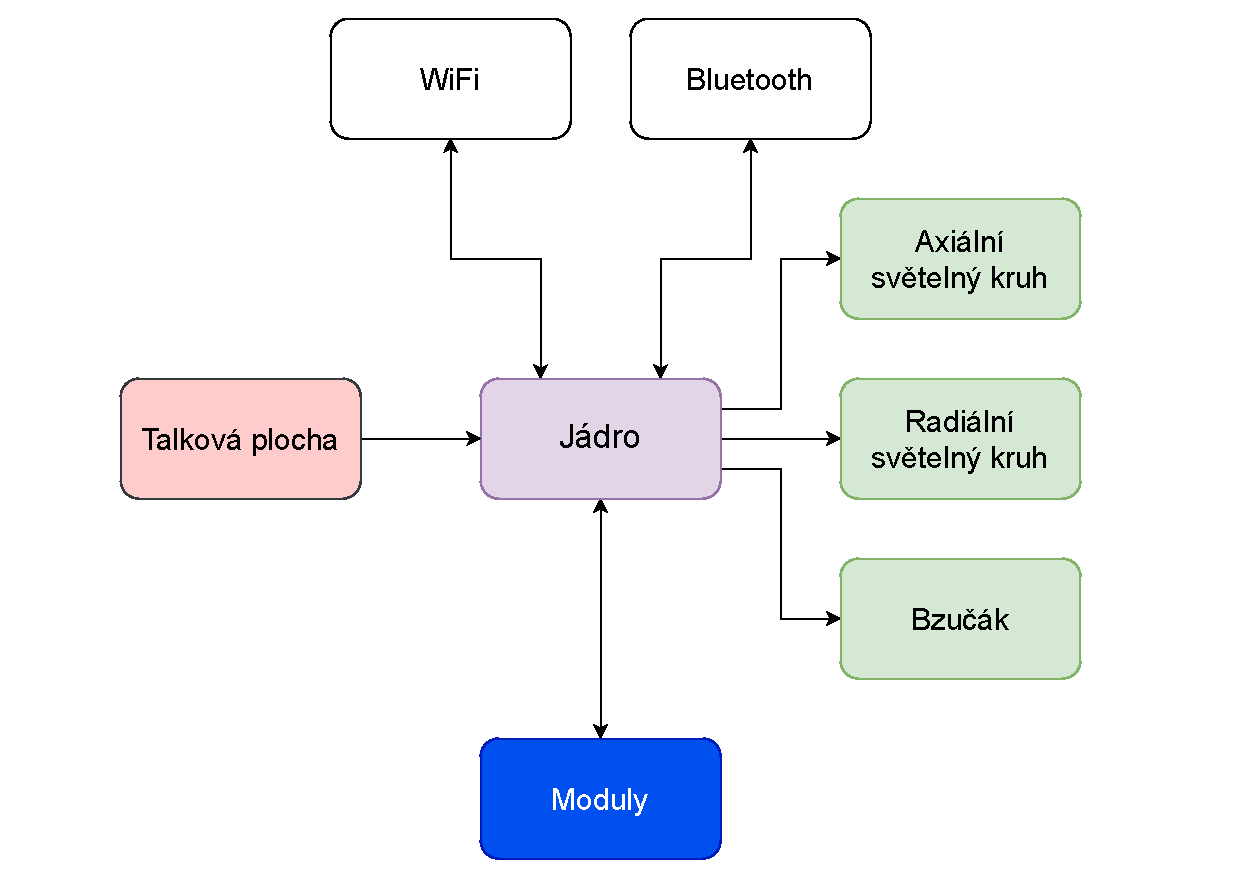
\includegraphics[width=0.65\textwidth]{text/TeoretickyUvod/AplikaceHernichZarizeni/diagram/zanoreni_1.pdf}
    \caption{Základního blokové schéma zařízení}
    \label{fig:diagram_zanoreni_1}
\end{figure}

\vspace{-10mm}
\section{Moduly}
Základní řídící jednotka je tedy schopná poskytnout základní funkce, které jsou potřeba pro většinu her.
Některé hry ale mohou vyžadovat nějakou specifickou funkci, kterou základní zařízení nedokáže poskytnout.
Proto je vhodné, aby bylo možné k základnímu zařízení připojit externí moduly, bez kterých by se konkrétní hry neobešli.

Jedním z takových modulů může být například modul dvířka, který umožní do zařízení uložit nějaký objekt a vydat jej jen po nějaké interakci.
Konkrétně má takový modul několik samostatných zamykatelných přihrádek, které se dají samostatně ovládat a mohou sloužit např. pro více týmů nebo uchovávat více objektu do různých částí hry.

Jednoduchá hrou která vyžaduje modul dvířka je např. hra Maják. %%TODO: vymyslet lepčí název tohle se  mi moc nepozdává (je to název z her od Petra na první lucerný v roce 2021)
V této hře jsou hráči rozděleni do týmů a každý tým má svou barvu, od které je odvozena konkrétní přihrádka. 
Týmy mají za úkol získat co nejvíc sad kartiček.
Na hřišti je několik automatických stanovišť s modulem dvířka a v každém z nich je nějaký typ kartičky.
Každé stanoviště během hry umožňuje přístup právě jednomu týmu, které v pravidelném intervalu mění a čas do změny reprezentuje na jednom z kruhů.
Při startu hry si každé stanoviště náhodně vybere tým kterým začne a následně se už drží konstantního pořadí.
Když někdo dorazí ke stanovišti ve chvíli kdy má stanoviště zpřístupnění jeho tým a klepne na tlakovou plochu, stanoviště mu vydá kartičku.
Stanoviště se týmu zpřístupní jen v čase daného týmu a navíc jen jednou za kolo.
Hráčům cíleně není představen celí mechanizmus výdeje kartiček, je jim řečeno jen že se přihrádka otevírá klepnutím do tlakové plochy a že je zajímají jen kartičky jejich barvi. 
Tým tedy musí spolupracovat nejprve na odhalení mechanizmu a následně myslet jak tedy zvítězit.

Podobná hra se duď dá hrát samostatně nebo muže jít například jen o metodu jak získávat suroviny v nějaké komplexnější hře.

Další modul, který se dá připojit je zvukový modul.
Hra který vyžaduje zvukový modul je například hra s názvem Ticho.
Tato hrá vyžaduje zároveň i modul dvířka.
V této hře stanoviště sleduje intenzitu zvuku v okoli a v momente kdy hluk klesne pod stanovenou úroveň stanoviště otevře dvířka. 
% Ucastnikum není ovládání představeno a musí tak na něj přijít samy.
Stanoviště je hráčům představeno jako "magicka krabicka" za carou ke ktere se nesmi proplížit ale muzou ji z dalky ovlivnit.
Ukolem hracu tak bylo prijit na to jak lucerna funguje a jak ji presvedci aby se otevřela.

V rámci zvukového modulu je i možnost přehrát nějakou nahrávku.
Tato část zvukového modulu umožňuje intenzivnější vtažení hráče do hry s příběhem.
Může jít například o unikovou hru při které hráč ocitne v oblasti v neznámém bludišti a jeho úkolem je najít cestu ven.
Při hledání muže narazit na různá stanoviště která mu nejprve přehrají nějakou část příběhu a následně mu dají nějaký úkol nebo radu jak postupovat dál.

Podstatným modulem je také komunikační modul který umožňuje připojení k mobilní síti a tím i komunikaci s ostatními zařízeními na velkou vzdálenost.
Tento modul je potřeba například pro hru Zábor kopce.

V této hře se na hřišti o velké rozloze nachází několik automatických stanovišť.
Hráči jsou rozděleni do týmů a každý tým má svou barvu a své tlačítko na stanovišti označené barvou týmu.
V hře Zábor Kopce je hlavním cílem získávat body pro svůj tým ovládnutím a udržením stanovišť na rozsáhlém hřišti. 
Axiálním světelný kruh zobrazuje rozdělení tlakové plochu na jednotlivá tlačítka týmů podle jejich barvi.
Zabrání stanoviště pak mohou hráči provést stiskem příslušného tlačítka. 
Získávání bodů se odehrává dvěma způsoby, ovládnutím stanoviště a následným držením stanoviště pod kontrolou. 
Týmy mohou přebírat stanoviště od soupeřů, což přidává hře strategický rozměr. 
Výhodou je kontrolovat více stanovišť najednou, což umožňuje rychlejší získávání bodů a zvyšuje šanci na vítězství.
Komunikační modul je tu potřebný pro vyhodnocování hry.
Stanoviště totiž musí být schopné komunikovat s centrálním serverem, který vyhodnocuje hru a zobrazuje její průběh.
Tato hra je původně navržena pro airsoftové hráče na hřiště v Mokra-Horakov o rozloze \(6.7\-[ha]\) \cite{MokraHorakov}.
V takovém prostředí je tedy komunikace pomocí WiFi či Bluetooth nedostačuje, protože stanoviště mohou být i několik set metrů od sebe.

\subsection{Výběr bezdrátové komunikace dlouhého dosahu}
Pro komunikaci na dlouhé vzdálenosti se nabízí asi jen dvě základní možnosti, LoRa a mobilní síť.
Ještě počátkem roku 2023 by byla i třetí možnost, Sigfox, ale jeho síť byla v ČR vypnuta \cite{SigfoxKonci}.

LoRa je technologie určená pro komunikaci na dlouhé vzdálenosti s malou spotřebou a datovou propustností.
Pracuje v bezlicenčním pásmu a není tedy třeba platit za provoz.
Její dosah je i v zastavěné oblasti v řádu kilometru \cite{LoRaSEMTECH}, a za ideálních podmínek na přímou viditelnost i přes sto kilometru \cite{LoRaEMAN}. 
Nevýhoda LoRy je ale malá datová propustnost ještě snížená omezením času provozu na \(1\-\%\)\cite{LoRaEMAN}.

Mobilní síď má v porovnání s LoRou výrazně větší datovou propustnost, ale na druhou stranu je třeba platit za provoz a je méně energeticky úsporná.
Například NB-IoT je energeticky asi o třetinu náročnější než LoRa.
Přesto je dostatečně úsporná aby bylo zařízení, které tuto technologii využívá, sto běžet na baterii přes deset let \cite{LoRaVSNB-IoT}.
Energetická náročnost tedy není problém a vyšší datová propustnost společně s připojením na internet je významnější výhoda než bezplatný provoz u LoRy.
Další výhodou LoRy by mohla být nezávislost na pokrytí mobilní sítí, ale vzhledem k tomu, že pokrytí NB-IoT sítě je v ČR údajně \(100\-\%\)\cite{NB-IoTPokryti}, není tento fakt důležitý. 

\newpage
\section{Dynamických zařízení}
U některých her je potřeba, aby měl měl hráč nějaké zařízení které bude moci nosit s sebou a které mu při hře bude sloužit jako identifikace a nástroj pro plnění úkolu.
Takové zařízení by mělo být co nejmenší a co nejlehčí, aby hráče při hře nezdržovalo.
Navíc by mělo být co nejlevnější aby tolik nevadilo když jej některý hráč třeba ztratí, což se přeci jen může stát.
Mimo to toto zařízení musí být sto zobrazit svuj stav a převzít od uživatele jednoduchý pokyn.

Rozhodli jsme že toto zařízení bude svuj stav zobrazovat pomocí pěti inteligentních RGB LED a jako vstup mu budou sloužit dvě tlačítka.
Abychom nemuseli řešit napájení má toto zařízení USB konektor a je určeno k napájení powerbankou.
Toto zařízení jsme nazvali SemiSemafor a jeho vzhled je na obrázku \ref{fig:SemiSemafor}.

\begin{figure}[h]
    \centering
    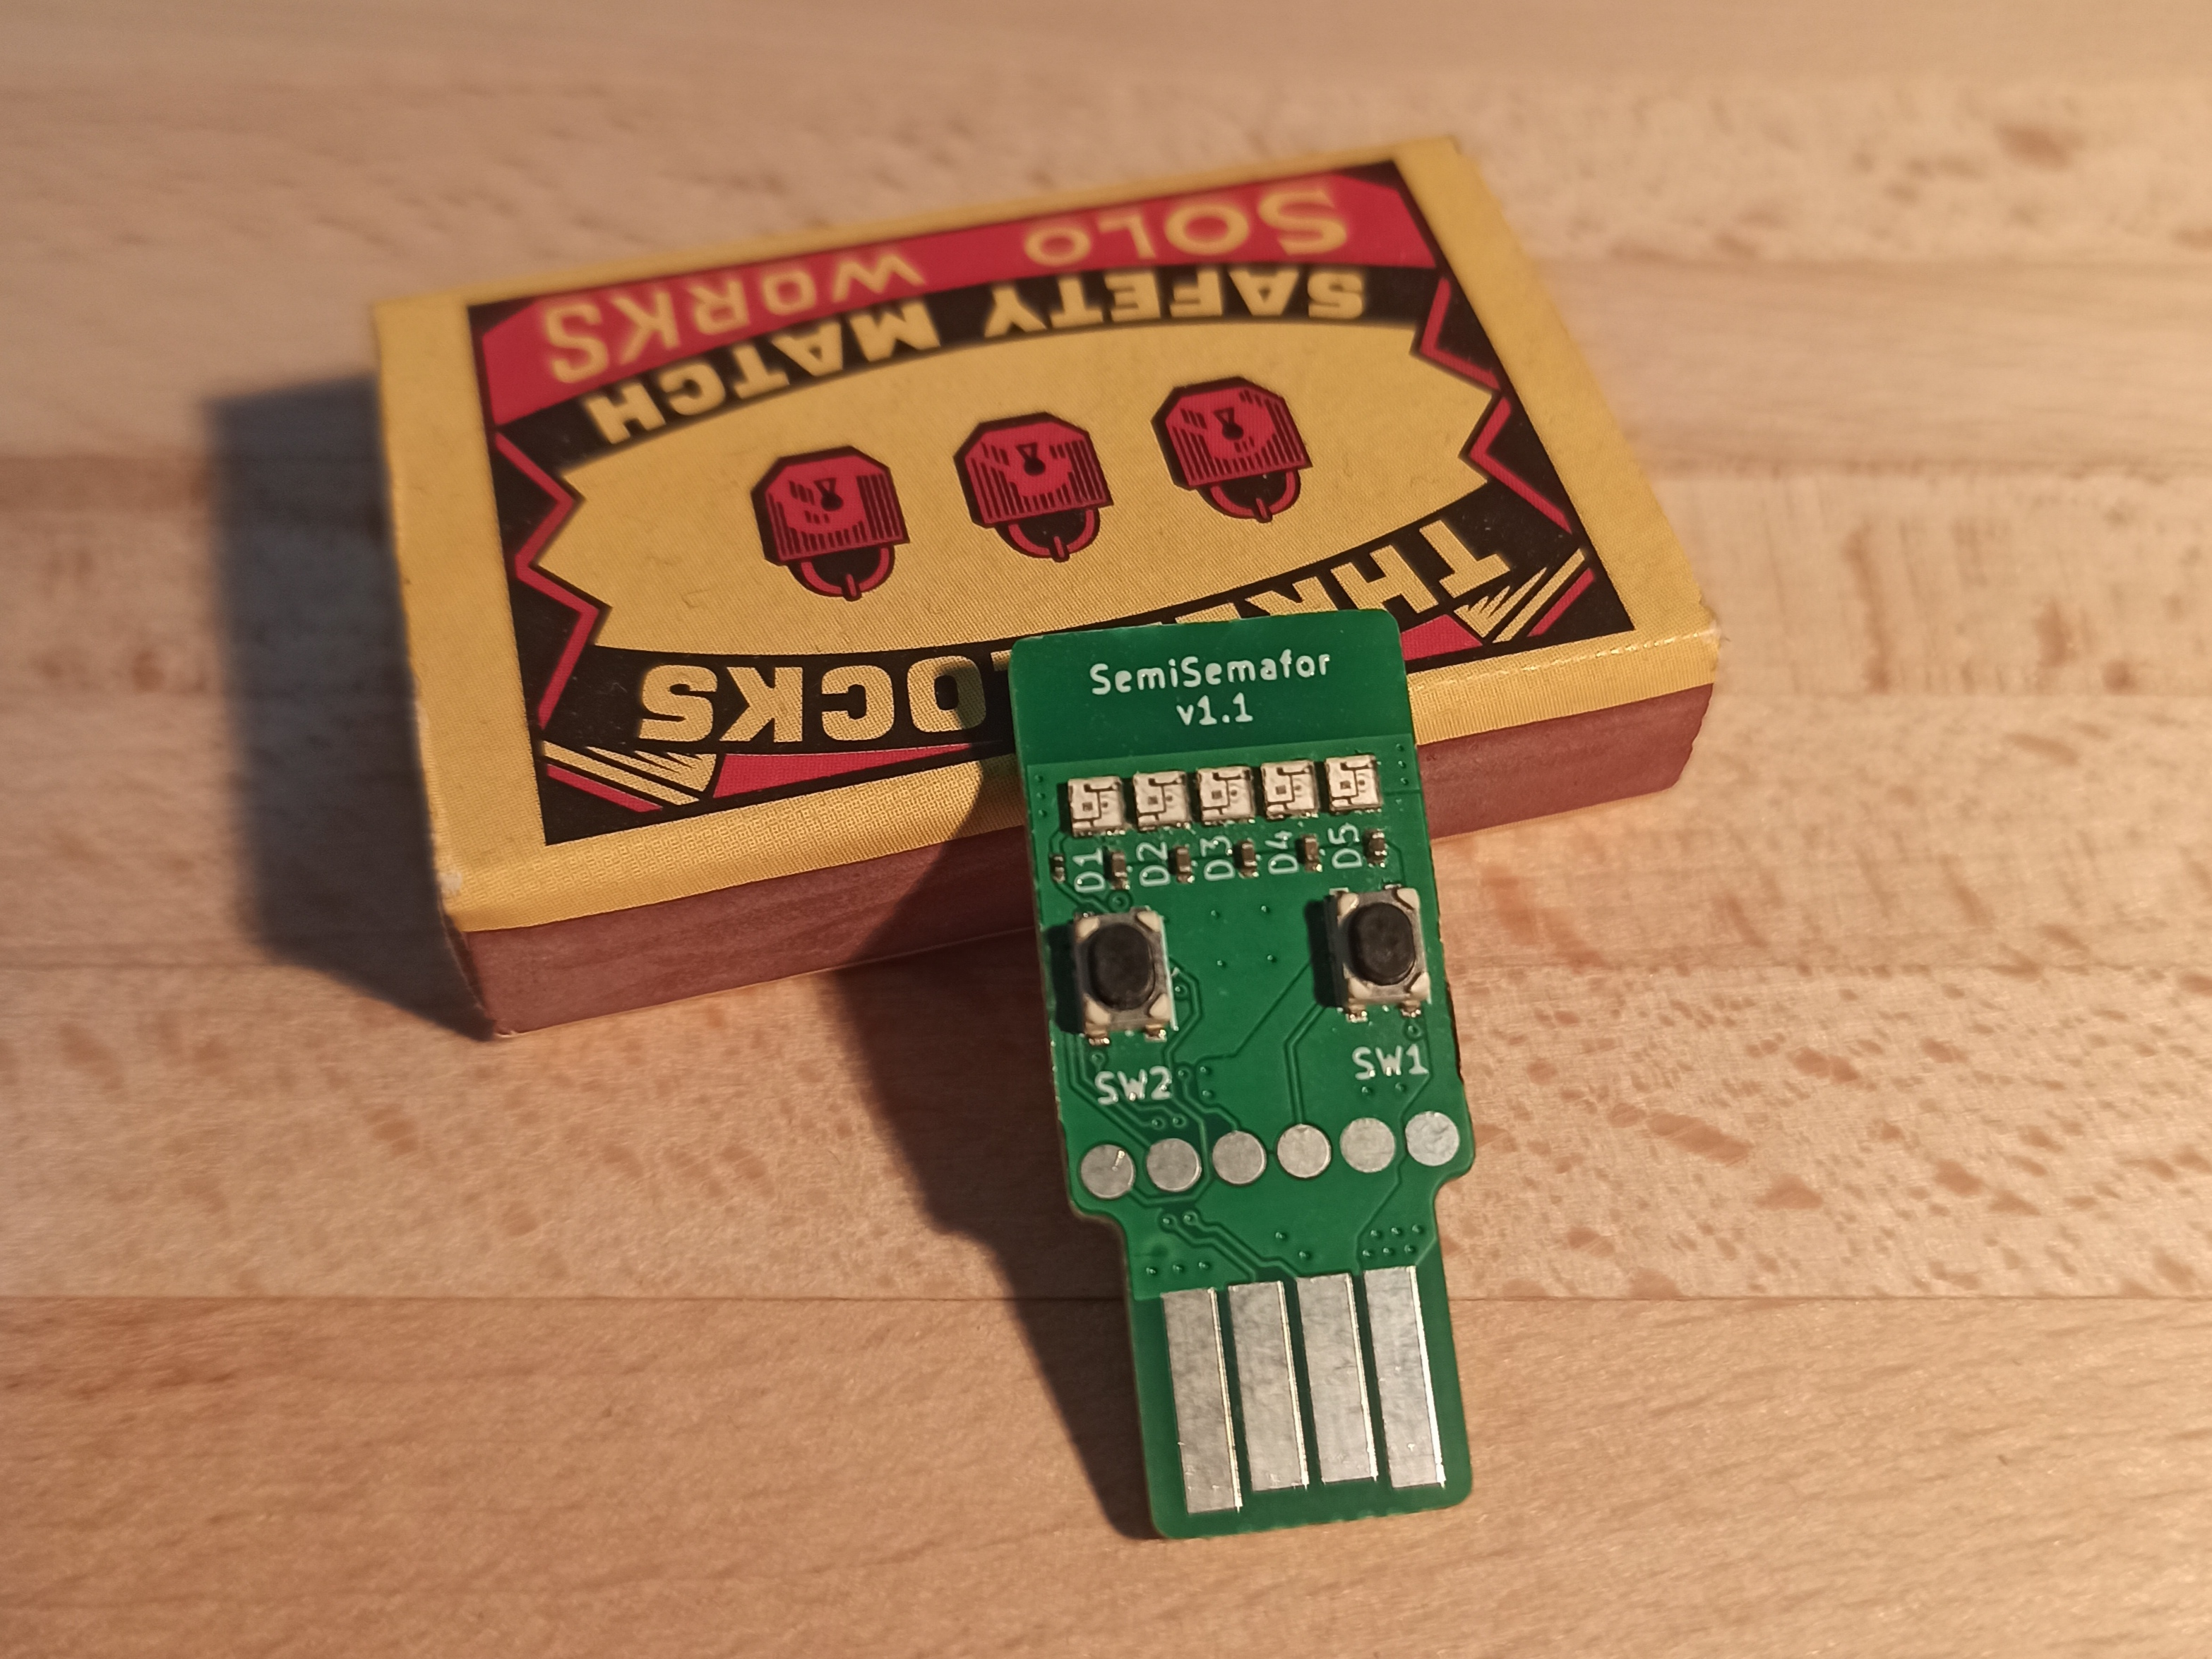
\includegraphics[width=0.8\textwidth]{text/TeoretickyUvod/AplikaceHernichZarizeni/img/1702085190411.jpg}
    \caption{Zařízení SemiSemafor}
    \label{fig:SemiSemafor}
\end{figure}

\subsection{Využití zařízení SemiSemafor}
SemiSemabor je využitelný například ve hře s názvem Duchové.

